%!TEX root = ../main.tex

\begin{frame}[t]\frametitle{Git Concepts}
	Now that you have been introduced to Git, let's clarify
	some of the concepts you have encountered.

	\begin{figure}[h!]
	    \label{states}\vspace{0.2cm}
	        \scalebox{0.35}{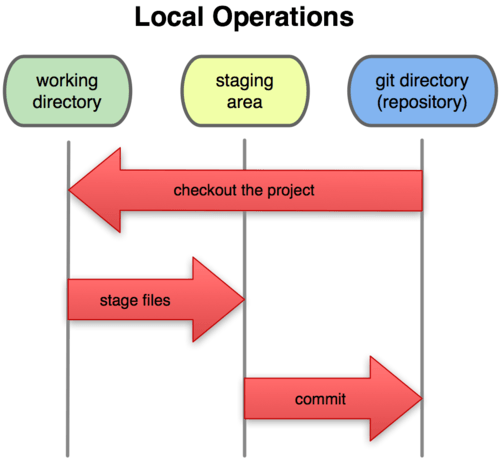
\includegraphics{figures/git-states}}            
    \end{figure}
\end{frame}

\begin{frame}[t]\frametitle{Git Concepts}
	We have also seen the various ways Git recognizes and
	records information about files.

	\begin{figure}[h!]
	    \label{file-states}\vspace{0.2cm}
	        \scalebox{0.55}{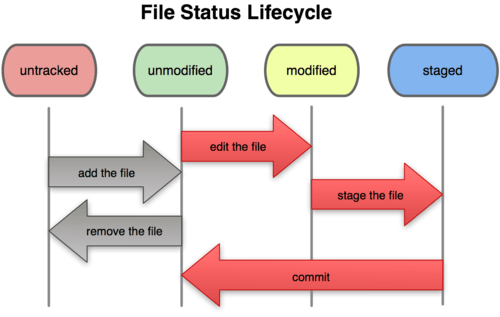
\includegraphics{figures/file-states}}            
    \end{figure}
\end{frame}

\begin{frame}[t]\frametitle{Git Concepts}
	Tracking:
	\begin{itemize}
		\item Git will only track files you tell it to track
		\item Only tracked files have a commit history, enabling:
		\begin{itemize}
			\item updates to remote repositories
			\item reverting changes
		\end{itemize}
	\end{itemize}
\end{frame}

\begin{frame}[t,fragile]\frametitle{Git Concepts}
	Let's see how Pam begins tracking ``File d'', which she
	just created and added to her project. 
	Her working directory looks like this:

    \begin{center}
        \tikzstyle{file}=[draw, rectangle, text centered, text width=2.5cm,
            fill=black!20, rounded corners]
        \resizebox{6cm}{6cm}{%
        \begin{tikzpicture}

            \begin{scope}[local bounding box=bb]
                \node (server) {Pam's Computer};
                \node [file, below of=server] (folder) {MyProject/};
                \node [file,below of=folder,xshift=2cm] (a) {File a};
                \node [file,below of=a] (b) {File b};
                \node [file,below of=b] (c) {File c};
                \node [file,below of=c,fill=white] (d) {File d};
                \node [file,below of=d,xshift=-2cm] (git) {.git/};
                \node [below of=git,xshift=0.3cm] (content) {...};

                \draw (folder) -- (0,-3);
                \draw (0,-3) -- (a.west);
                \draw (0,-3) -- (b.west);
                \draw (0,-3) -- (c.west);
                \draw (0,-3) -- (d.west);
                \draw (0,-3) -- (git.north);
                \draw (git.south) -- (content.west);
            \end{scope}

            \begin{pgfonlayer}{background}
                \node [fill=blue!20,fit=(bb)] {};
            \end{pgfonlayer}

            \node [right of=d,node distance=4cm] (track) {Untracked File};
            \draw [<-] (d.east) -- (track.west);

        \end{tikzpicture}
        }
    \end{center}
\end{frame}

\begin{frame}[t,fragile]\frametitle{Git Concepts}
	Pam opens terminal and issues the following command:

	\vspace{0.5cm}
	\inlinecode{\$ git add ``File d''}

    \begin{center}
        \tikzstyle{file}=[draw, rectangle, text centered, text width=2.5cm,
            fill=black!20, rounded corners]
        \resizebox{5.5cm}{5.5cm}{%
        \begin{tikzpicture}

            \begin{scope}[local bounding box=bb]
                \node (server) {Pam's Computer};
                \node [file, below of=server] (folder) {MyProject/};
                \node [file,below of=folder,xshift=2cm] (a) {File a};
                \node [file,below of=a] (b) {File b};
                \node [file,below of=b] (c) {File c};
                \node [file,below of=c,fill=red!70] (d) {File d};
                \node [file,below of=d,xshift=-2cm] (git) {.git/};
                \node [below of=git,xshift=0.3cm] (content) {...};

                \draw (folder) -- (0,-3);
                \draw (0,-3) -- (a.west);
                \draw (0,-3) -- (b.west);
                \draw (0,-3) -- (c.west);
                \draw (0,-3) -- (d.west);
                \draw (0,-3) -- (git.north);
                \draw (git.south) -- (content.west);
            \end{scope}

            \begin{pgfonlayer}{background}
                \node [fill=blue!20,fit=(bb)] {};
            \end{pgfonlayer}

            \node [right of=d,node distance=4cm,text width=3cm] (track) {Newly Tracked, Not Committed};
            \draw [<-] (d.east) -- (track.west);

        \end{tikzpicture}
        }
    \end{center}
\end{frame}

\begin{frame}[c,fragile]\frametitle{Git Concepts}
	Pam pushes her changes to the remote
	Central Server.

	\vspace{0.5cm}
	\newbox{\mybox}
	\begin{lrbox}{\mybox}
	\begin{minipage}{\linewidth}
	\begin{lstlisting}[basicstyle=\footnotesize\ttfamily\color{white}]
	$ git commit -m "Added File d, contains info on fat%."
	$ git push origin master
	\end{lstlisting}
	\end{minipage}
	\end{lrbox}
	\colorbox{black}{\usebox{\mybox}}
\end{frame}

\begin{frame}[c]
    \begin{center}
        \Large Collaboration with Git
    \end{center}
\end{frame}

\begin{frame}[t,fragile]\frametitle{Git Concepts}
	David wishes to update his local files with the most
	recent version from the Central Server (i.e. fast-forwarding
	to Pam's commit.)

	\begin{center} 
		\begin{figure}[h!] \centering
			\subfloat{
		\tikzstyle{file}=[draw, rectangle, text centered, text width=2.5cm,
            fill=black!20, rounded corners]
        \resizebox{3cm}{5cm}{%
        \begin{tikzpicture}

            \begin{scope}[local bounding box=bb]
                \node (server) {Central Server};
                \node [file, below of=server] (folder) {MyProject/};
                \node [file,below of=folder,xshift=2cm] (a) {File a};
                \node [file,below of=a] (b) {File b};
                \node [file,below of=b] (c) {File c};
                \node [file,below of=c] (d) {File d};
                \node [file,below of=d,xshift=-2cm] (git) {.git/};
                \node [below of=git,xshift=0.3cm] (content) {...};
                \node [below of=content] (commit) {17a10ca55};

                \draw (folder) -- (0,-3);
                \draw (0,-3) -- (a.west);
                \draw (0,-3) -- (b.west);
                \draw (0,-3) -- (c.west);
                \draw (0,-3) -- (d.west);
                \draw (0,-3) -- (git.north);
                \draw (git.south) -- (content.west);
            \end{scope}

            \begin{pgfonlayer}{background}
                \node [fill=blue!20,fit=(bb)] {};
            \end{pgfonlayer}

        \end{tikzpicture}
        }	
			         } 
			\subfloat{
		\tikzstyle{file}=[draw, rectangle, text centered, text width=2.5cm,
            fill=black!20, rounded corners]
        \resizebox{3cm}{5cm}{%
        \begin{tikzpicture}

            \begin{scope}[local bounding box=bb]
                \node (server) {David's Computer};
                \node [file, below of=server] (folder) {MyProject/};
                \node [file,below of=folder,xshift=2cm] (a) {File a};
                \node [file,below of=a] (b) {File b};
                \node [file,below of=b] (c) {File c};
                \node [file,below of=c,xshift=-2cm] (git) {.git/};
                \node [below of=git,xshift=0.3cm] (content) {...};
				\node [below of=content] (commit) {24b9da655};

                \draw (folder) -- (0,-3);
                \draw (0,-3) -- (a.west);
                \draw (0,-3) -- (b.west);
                \draw (0,-3) -- (c.west);
                \draw (0,-3) -- (git.north);
                \draw (git.south) -- (content.west);
            \end{scope}

            \begin{pgfonlayer}{background}
                \node [fill=blue!20,fit=(bb)] {};
            \end{pgfonlayer}

        \end{tikzpicture}
        }	
			         } \         
		\end{figure}
	\end{center}

	Commit History:

	... $\rightarrow$ \colorbox{black!30}{24b9da655} $\rightarrow$ \colorbox{black!30}{75b10da55} $\rightarrow$ \colorbox{black!30}{17a10ca55}

\end{frame}

\begin{frame}[c]\frametitle{Git Concepts}
	When David issues the command 

	\vspace{0.5cm}
	\inlinecode{\$ git pull origin}

	\vspace{0.5cm}
	the changes upstream are \href{http://git-scm.com/book/en/Git-Basics-Working-with-Remotes}{fetched} from the Central Server and 
	merged with the files in his repository.
\end{frame}

\begin{frame}[c]
    \begin{center}
        \Large Branching
    \end{center}
\end{frame}

\begin{frame}[c]\frametitle{Git Concepts}
	Up until now, we have glossed over one very important feature
	of Git: \framebox{branching}. 

	\vspace{1cm}
	But we have learned two concepts: 
	the \framebox{commit} and 
	\framebox{git repository}. 
\end{frame}

\begin{frame}[c]\frametitle{Git Concepts}
	A Git \framebox{branch} is just a
	\textbf{pointer to a specific commit.}

	\begin{itemize}
		\item allows for non-linear workflows
		and simultaneous channels of development.
		\item aids the implemention new features.
	\end{itemize}

\end{frame}

\begin{frame}[c]\frametitle{Git Concepts}
	An economist might use \framebox{branching} to:

	\begin{itemize}
		\item Attempt a new identification strategy
		\item Quickly revert to a previous set of results
		\item Experiment with new numerical software
	\end{itemize}
\end{frame}

\begin{frame}[t]\frametitle{Git Concepts}
	Git repositories, commits and branches all describe
	a location in Gitland.

	\begin{center} 
		\begin{figure}[h!] \centering
			\subfloat{
		\tikzstyle{commit}=[draw, rectangle, text centered, text width=0.5cm,
            fill=green!20, rounded corners]
		\tikzstyle{branch}=[draw, rectangle, text centered, text width=1cm,
            fill=white, rounded corners]
        \resizebox{5cm}{5cm}{%
        \begin{tikzpicture}

            \begin{scope}[local bounding box=bb]
                \node (server) {Pam's Repository};
                \node [commit,below of=server] (c1) {C1};
                \node [commit,below of=c1] (c2) {C2};
                \node [commit,below of=c2] (c3) {C3};
                \node [commit,below of=c3] (c6) {C6};
                \node [commit,right of=c3,xshift=1cm] (c4) {C4};
                \node [commit,below of=c4] (c5) {C5};
                \node [branch,left of=c6,xshift=-0.5cm] (master) {master};
                \node [branch,right of=c5,xshift=0.5cm] (dev) {dev};
                \node [branch,above of=dev,rounded corners=false] (head) {HEAD};

                \draw [->] (c1) -- (c2);
                \draw [->] (c2) -- (c3);
                \draw [->] (c3) -- (c4);
                \draw [->] (c3) -- (c6);
                \draw [->] (c4) -- (c5);
                \draw [->,very thick] (master) -- (c6);
                \draw [->,very thick] (dev) -- (c5);
                \draw [->,very thick] (head) -- (dev);
            \end{scope}

            \begin{pgfonlayer}{background}
                \node [fill=blue!20,fit=(bb)] {};
            \end{pgfonlayer}

        \end{tikzpicture}
        }	
			         } 
			\subfloat{
		\tikzstyle{file}=[draw, rectangle, text centered, text width=2.5cm,
            fill=black!20, rounded corners]
        \resizebox{3cm}{5cm}{%
        \begin{tikzpicture}

            \begin{scope}[local bounding box=bb]
                \node (server) {Pam's HEAD Pointer};
                \node [file, below of=server] (folder) {MyProject/};
                \node [file,below of=folder,xshift=2cm] (a) {File a};
                \node [file,below of=a] (b) {File b};
                \node [file,below of=b] (c) {File c};
                \node [file,below of=c,xshift=-2cm] (git) {.git/};
                \node [below of=git,xshift=0.3cm] (content) {...};
				\node [below of=content] (commit) {24b9da655};

                \draw (folder) -- (0,-3);
                \draw (0,-3) -- (a.west);
                \draw (0,-3) -- (b.west);
                \draw (0,-3) -- (c.west);
                \draw (0,-3) -- (git.north);
                \draw (git.south) -- (content.west);
            \end{scope}

            \begin{pgfonlayer}{background}
                \node [fill=blue!20,fit=(bb)] {};
            \end{pgfonlayer}

        \end{tikzpicture}
        }	
			         } \         
		\end{figure}
	\end{center}
\end{frame}

\begin{frame}[c]\frametitle{Git Concepts}
	\framebox{HEAD} is a special pointer which always
	points to the current focal branch. \framebox{master}
	and \framebox{dev} are branches, which merely point
	to a particular \framebox{commit}. Each 
	\framebox{commit} is a saved state, or snapshot 
	of your project \emph{as a whole}.
\end{frame}

\begin{frame}[c]\frametitle{Git Concepts}
	Navigate Gitland by changing the location of the
	\framebox{HEAD} pointer. You can checkout
	a branch:

	\vspace{0.5cm}
	\inlinecode{\$ git checkout master}

	\vspace{0.5cm}
	\tikzstyle{commit}=[draw, rectangle, text centered, text width=0.5cm,
        fill=green!20, rounded corners]
	\tikzstyle{branch}=[draw, rectangle, text centered, text width=1cm,
        fill=white, rounded corners]
    \resizebox{5cm}{5cm}{%
    \begin{tikzpicture}

        \begin{scope}[local bounding box=bb]
            \node (server) {Pam's Repository};
            \node [commit,below of=server] (c1) {C1};
            \node [commit,below of=c1] (c2) {C2};
            \node [commit,below of=c2] (c3) {C3};
            \node [commit,below of=c3] (c6) {C6};
            \node [commit,right of=c3,xshift=1cm] (c4) {C4};
            \node [commit,below of=c4] (c5) {C5};
            \node [branch,left of=c6,xshift=-0.5cm] (master) {master};
            \node [branch,right of=c5,xshift=0.5cm] (dev) {dev};
            \node [branch,above of=master,rounded corners=false] (head) {HEAD};

            \draw [->] (c1) -- (c2);
            \draw [->] (c2) -- (c3);
            \draw [->] (c3) -- (c4);
            \draw [->] (c3) -- (c6);
            \draw [->] (c4) -- (c5);
            \draw [->,very thick] (master) -- (c6);
            \draw [->,very thick] (dev) -- (c5);
            \draw [->,very thick] (head) -- (master);
        \end{scope}

        \begin{pgfonlayer}{background}
            \node [fill=blue!20,fit=(bb)] {};
        \end{pgfonlayer}

    \end{tikzpicture}
    }
\end{frame}

\begin{frame}[c]
    \begin{center}
        \Large Merging
    \end{center}
\end{frame}

\begin{frame}[c]\frametitle{Git Concepts}
	We will not get into the details of merging, but
	we can explore one example. Let's have Pam merge
	the \framebox{dev} branch into \framebox{master}. 

	\vspace{0.5cm}
	\inlinecode{\$ git merge dev}
\end{frame}

\begin{frame}[c]\frametitle{Git Concepts}
	If the \framebox{master} and \framebox{dev} branches
	did not modify the same file, the merge should go smoothly,
	producing an automatic merge commit.
	Otherwise, Pam has to modify the conflicted file(s)
	and then manually commit. 
\end{frame}

\begin{frame}[fragile]
    \frametitle{Git Concepts}
    Let's say Pam has a merge conflict. The conflicted file
    looks like this in the two different branches.

    \begin{itemize}
        \item \framebox{dev}

        \vspace{0.25cm}
        \newbox{\mybox}
        \begin{lrbox}{\mybox}
        \begin{minipage}{\linewidth}
        \begin{lstlisting}[basicstyle=\tiny\ttfamily\color{white}]
places = {'Mexico':'Spanish', 'United States':'English',
    'Brazil':'Portuguese'}

for key in places:
        print key, places[key]

for i in [1,2,3]:
        print i
        \end{lstlisting}
        \end{minipage}
        \end{lrbox}
        \colorbox{black}{\usebox{\mybox}}

        \vspace{0.25cm}
        \item \framebox{master}

        \vspace{0.25cm}
        \newbox{\mybox}
        \begin{lrbox}{\mybox}
        \begin{minipage}{\linewidth}
        \begin{lstlisting}[basicstyle=\tiny\ttfamily\color{white}]
places = {'Mexico':'Spanish', 'United States':'English',
    'Brazil':'Portuguese'}

for key in places:
        print key, places[key]

for i in [4,5,6]:
    print i
        \end{lstlisting}
        \end{minipage}
        \end{lrbox}
        \colorbox{black}{\usebox{\mybox}}
        
    \end{itemize}

\end{frame}

\begin{frame}[fragile]\frametitle{Git Concepts}
    After attempting the merge, Git forces Pam to resolve
    all merge conflicts. Git modifies the file in her working
    directory to highlight the conflicting portions of the file.

    \vspace{0.5cm}
    \newbox{\mybox}
    \begin{lrbox}{\mybox}
    \begin{minipage}{\linewidth}
    \begin{lstlisting}[basicstyle=\tiny\ttfamily\color{white}]
places = {'Mexico':'Spanish', 'United States':'English',
        'Brazil':'Portuguese'}

for key in places:
        print key, places[key]

<<<<<<< HEAD
for i in [4,5,6]:
=======
for i in [1,2,3]:
>>>>>>> new
        print i
    
    \end{lstlisting}
    \end{minipage}
    \end{lrbox}
    \colorbox{black}{\usebox{\mybox}}

    \vspace{0.5cm}
    \inlinecode{<<<<<<<< HEAD} signals the version of your current branch
    and \inlinecode{>>>>>>>> new} that of the branch you attempting to 
    merge into your current branch. 
\end{frame}

\begin{frame}[fragile]\frametitle{Git Concepts}
    Pam resolves the conflict by editing the file.

    \vspace{0.5cm}
    \newbox{\mybox}
    \begin{lrbox}{\mybox}
    \begin{minipage}{\linewidth}
    \begin{lstlisting}[basicstyle=\tiny\ttfamily\color{white}]
places = {'Mexico':'Spanish', 'United States':'English',
        'Brazil':'Portuguese'}

for key in places:
        print key, places[key]

for i in [1,2,3,4,5,6]:
        print i
    \end{lstlisting}
    \end{minipage}
    \end{lrbox}
    \colorbox{black}{\usebox{\mybox}}

    \vspace{0.5cm}
    Then she commits again.

    \vspace{0.5cm}
    \newbox{\mybox}
    \begin{lrbox}{\mybox}
    \begin{minipage}{\linewidth}
    \begin{lstlisting}[basicstyle=\tiny\ttfamily\color{white}]
$ git add filea
$ git commit -m "Resolved conflict, iterating through long list"
    \end{lstlisting}
    \end{minipage}
    \end{lrbox}
    \colorbox{black}{\usebox{\mybox}}
\end{frame}

\begin{frame}[t]\frametitle{Git Concepts}
    After the merge is complete, Pam's commit history in
    her local repository looks like:

    \vspace{0.5cm}
    \tikzstyle{commit}=[draw, rectangle, text centered, text width=0.5cm,
        fill=green!20, rounded corners]
    \tikzstyle{branch}=[draw, rectangle, text centered, text width=1cm,
        fill=white, rounded corners]
    \resizebox{5cm}{5cm}{%
    \begin{tikzpicture}

        \begin{scope}[local bounding box=bb]
            \node (server) {Pam's Repository};
            \node [commit,below of=server] (c1) {C1};
            \node [commit,below of=c1] (c2) {C2};
            \node [commit,below of=c2] (c3) {C3};
            \node [commit,below of=c3] (c6) {C6};
            \node [commit,right of=c3,xshift=1cm] (c4) {C4};
            \node [commit,below of=c4] (c5) {C5};
            \node [commit,below of=c6] (c7) {C7};
            \node [branch,left of=c7,xshift=-0.5cm] (master) {master};
            \node [branch,right of=c5,xshift=0.5cm] (dev) {dev};
            \node [branch,above of=master,rounded corners=false] (head) {HEAD};
            

            \draw [->] (c1) -- (c2);
            \draw [->] (c2) -- (c3);
            \draw [->] (c3) -- (c4);
            \draw [->] (c3) -- (c6);
            \draw [->] (c4) -- (c5);
            \draw [->] (c6) -- (c7);
            \draw [->] (c5) -- (c7);
            \draw [->,very thick] (master) -- (c7);
            \draw [->,very thick] (dev) -- (c5);
            \draw [->,very thick] (head) -- (master);
        \end{scope}

        \begin{pgfonlayer}{background}
            \node [fill=blue!20,fit=(bb)] {};
        \end{pgfonlayer}

    \end{tikzpicture}
    }
\end{frame}

\begin{frame}[fragile]\frametitle{Git Concepts}
    To view the difference between this and the last
    commit, Pam uses the command 
    \inlinecode{\$ git diff HEAD^ -- filea}

    \begin{center} 
        \begin{figure}[h!] \centering
            \scalebox{0.45}{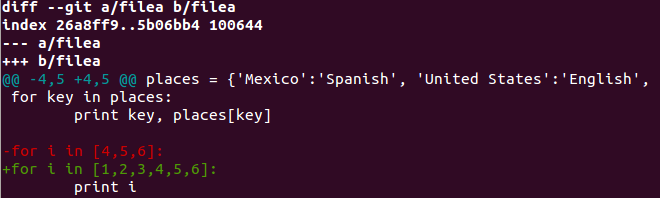
\includegraphics{figures/diff}}   
        \end{figure}
    \end{center}
\end{frame}

\begin{frame}[fragile]\frametitle{Git Concepts}
    Because she has 
    \href{http://stackoverflow.com/questions/3713765/viewing%
    -all-git-diffs-with-vimdiff}{configured} 
    Git to use a difftool, 
    she also uses vimdiff with the command
    \inlinecode{\$ git difftool HEAD^ -- filea}
    for a side-by-side comparison.

    \begin{center} 
        \begin{figure}[h!] \centering
            \scalebox{0.27}{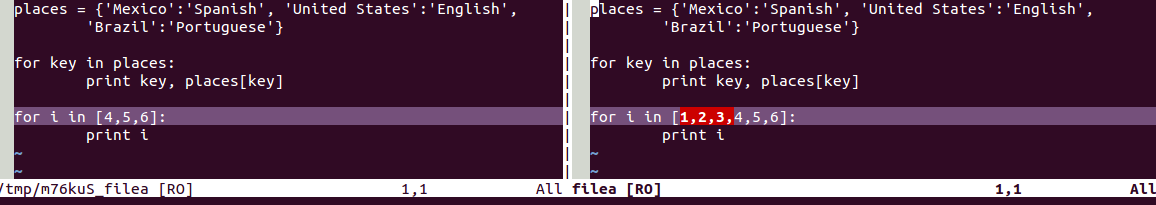
\includegraphics{figures/difftool}}   
        \end{figure}
    \end{center}
\end{frame}

\begin{frame}[c]
    \begin{center} \Large
        Framework For Understanding Git
    \end{center}
\end{frame}

\begin{frame}[c]\frametitle{Understanding Scope}

	\begin{itemize}
		\item Know the difference between
		\begin{itemize}
			\item git directory (i.e. Gitland)
			\item working directory (current, local state of files)
            \item
			The location of \framebox{HEAD} in your git directory
			and any local file modifications determine the state
			of your working directory
		\end{itemize}
	\end{itemize}
\end{frame}

\begin{frame}[t]\frametitle{Understanding the Commands}
		Commands fall under four categories:
		\begin{enumerate}
			\item Update your \textbf{working directory} to reflect
			a \textbf{git directory} 

			\vspace{0.3cm}
			\inlinecode{\$ git checkout master}
			
			\vspace{0.3cm}
			\item Update a \textbf{git directory} with another \textbf{git
			directory} 

			\vspace{0.3cm}
			\inlinecode{\$ git push origin master}
			
			\vspace{0.3cm}
			\item Update a \textbf{git directory} with your current
			\textbf{working directory} 

			\vspace{0.3cm}
			\inlinecode{\$ git commit}			

			\vspace{0.3cm}
			\item Update within a \textbf{git directory} 

			\vspace{0.3cm}
			\inlinecode{\$ git merge dev}
		\end{enumerate}
\end{frame}

\begin{frame}[t]\frametitle{Next Steps}
	We could not cover everything, here's how to proceed:

	\begin{itemize}
		\item Understanding how Git records file states or
		\href{http://git-scm.com/book/en/Getting-Started-Git-Basics}{snapshots}
		\item Creating and using git 
		\href{http://git-scm.com/book/en/Git-Branching-What-a-Branch-Is}{branches}
		\item \href{http://git-scm.com/book/en/Getting-Started-First-Time-Git-Setup}{Customizing} git
		\item Viewing differences across file versions 
		(i.e. \href{http://git-scm.com/book/en/Git-Basics-Recording-Changes-to-the-Repository}{diffing})
		\item \href{http://git-scm.com/book/en/Git-Basics-Undoing-Things}{Reverting} changes
	\end{itemize}
\end{frame}

\begin{frame}\frametitle{Comprehensive Resources}
    Many resources are available for git. 
    \href{http://stackoverflow.com/questions/tagged/git}{Stackoverflow} 
    will answer most questions. This 
    \href{http://stackoverflow.com/questions/315911/git-for-beginners-the-definitive-practical-guide}{post} is a great resource for beginners and advanced users alike.
\end{frame}

\begin{frame}
	Now \textbf{learn} Git so you can \textbf{forget} about
	versioning and move-on with research!
\end{frame}